\chapter{Waves}
	\section{Fundamentals of Waves} \index{Waves}

	You have probably heard of waves in the context of the ocean, a lake, or other bodies of liquid.  Waves are also found in earthquakes, sound, light, and even at the stadium when people do ``the wave.''  A \textit{wave} is a distortion that transfers energy from one place to another without the permanent transfer of mass. 
	
	The material that a wave travels through is called a \textit{medium}. \index{medium} \index{waves, medium} For instance, the medium for an ocean wave is water, while the medium for light could be air, glass, water, or even empty space (no medium).  
	\newpage
		\subsection{Types of Waves}
	 Waves can be categorized into several basic types: 
	\begin{itemize}
		\item \textit{Transverse Waves} - are waves that are displaced perpendicular to the direction of travel.  For instance, ocean waves are a type of transverse wave because their displacement is vertical, though they travel horizontally.
		Normally, a transverse wave is drawn similar to the figure below:
		\begin{center}
		\begin{figure}[h]
			\centering
			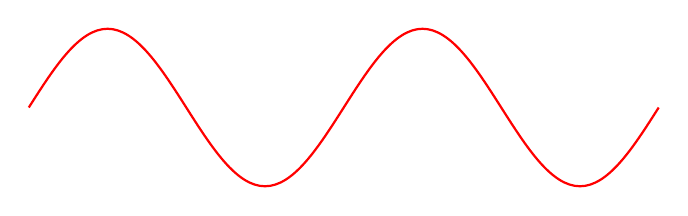
\begin{tikzpicture}

				 \draw[thick, red]
				 (3,0) sin (4,1) cos (5,0) sin (6,-1) cos (7,0)
				 sin (8,1) cos (9,0) sin (10,-1) cos (11,0);	
			 \end{tikzpicture}
			 \caption{A simple transverse wave}
		\end{figure}
		\end{center}	
		
		\item \textit{Longitudinal Waves} - are waves that are displaced in the same direction as the direction of travel.  You can think of this as a compression, or shock wave that travels through a medium.  The places where a material is closer together than normal are called compressions, while places that are spaced farther apart are called rarefractions, as seen in figure \ref{tester}
		
		\begin{figure}[h]
			\centering
			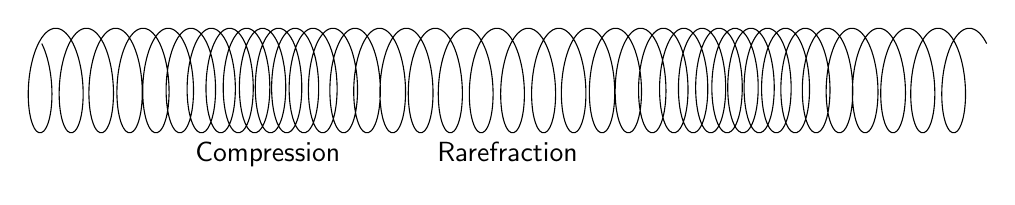
\begin{tikzpicture}[font=\sffamily] 
			\begin{scope}[z={(70:1)},y={(110:1)},local bounding box=coil] 
			\draw plot[domain=0:14400,variable=\t,samples=1441,smooth] 
			({\t/1200+0.1*pi*sin(\t/20)},{-0.5*sin(\t)},{0.5*cos(\t)}); 
			\end{scope} 
			\path (coil.south west) -- (coil.south east) 
			node[pos=0.25,below]{Compression} node[pos=0.5,below]{Rarefraction}; 
			
		\end{tikzpicture} 


			
			\caption{A simple longitudinal wave}
			\label{tester}
		\end{figure}	
		
		\item \textit{Electromagnetic Waves} - are waves that are made up of oscillating electric and magnetic fields.  These are usually modeled as transverse waves, but they are just representations of the strength of the electric and magnetic fields. 
		
		
		\begin{figure}[h]
			\centering
			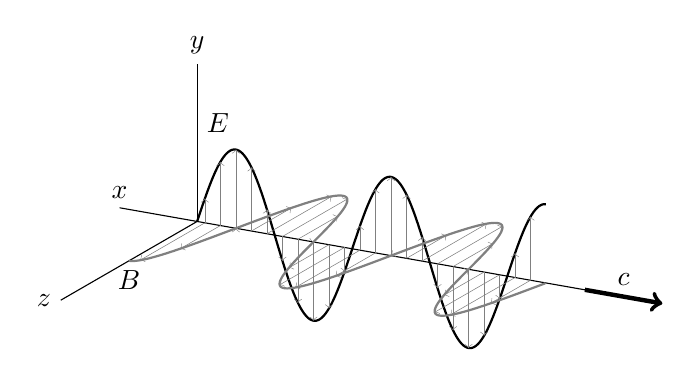
\begin{tikzpicture}[x={(-10:1cm)},y={(90:1cm)},z={(210:1cm)}]
			% Axes
			\draw (-1,0,0) node[above] {$x$} -- (5,0,0);
			\draw (0,0,0) -- (0,2,0) node[above] {$y$};
			\draw (0,0,0) -- (0,0,2) node[left] {$z$};
			% Propagation
			\draw[->,ultra thick] (5,0,0) -- node[above] {$c$} (6,0,0);
			% Waves
			\draw[thick] plot[domain=0:4.5,samples=200] (\x,{sin(deg(pi*\x))},0);
			\draw[gray,thick] plot[domain=0:4.5,samples=200] (\x,0,{cos(deg(pi*\x))});
			% Arrows
			\foreach \x in {0.1,0.3,...,4.4} {
				\draw[->,help lines] (\x,0,0) -- (\x,{sin(deg(pi*\x))},0);
				\draw[->,help lines] (\x,0,0) -- (\x,0,{cos(deg(pi*\x))});
			}
			% Labels
			\node[above right] at (0,1,0) {$\bm{E}$};
			\node[below] at (0,0,1) {$\bm{B}$};
			\end{tikzpicture}	
			\caption{An electromagnetic wave}
		\end{figure}
		 
		Electromagnetic Waves are what make up the Electromagnetic Spectrum.  Radio Waves, Microwaves, Infrared, Visible Light, Ultraviolet, X-rays and $\gamma$-rays are all electromagnetic waves.  They are categorized into different types based on their frequency. 
		 
	\end{itemize}

	There are other types of waves, such as matter waves and gravitational waves that are beyond the scope of this text.  

		\subsection{Basic Wave Characteristics and Vocabulary}
		
\begin{center}
	\begin{figure}[h]
		\centering
		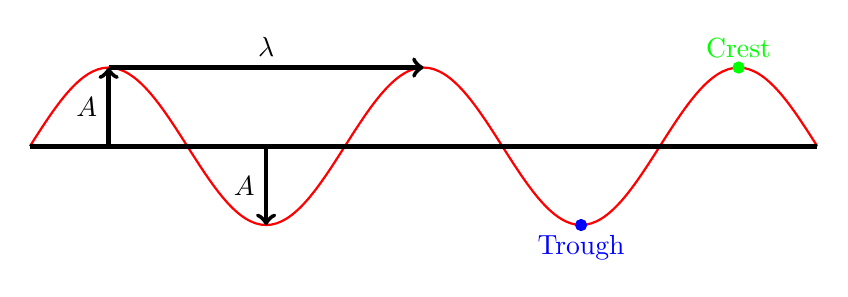
\begin{tikzpicture}
		
		\draw[thick, red]
		(3,0) sin (4,1) cos (5,0) sin (6,-1) cos (7,0)
		sin (8,1) cos (9,0) sin (10,-1) cos (11,0) sin (12,1) cos (13,0);	
			\draw[-,ultra thick] (3,0) --  (13,0);
			\draw[->,ultra thick] (4,1) -- node[above] {$\lambda$} (8,1);
			\draw[->,ultra thick] (4,0) -- node[left] {$A$} (4,1);
			\draw[->,ultra thick] (6,0) -- node[left] {$A$} (6,-1);
		 	\draw [blue] (10,-1) circle[radius=2pt] node[below] {Trough};
		 	\fill[blue] (10,-1)  circle[radius=2pt];
	 		\draw [green] (12,1) circle[radius=2pt] node[above] {Crest};
		 	\fill[green] (12,1)  circle[radius=2pt];
		 	
		\end{tikzpicture}
		\caption{The measurements of a wave}
		\label{fig:wavemeasure}
	\end{figure}
\end{center}	
		
	\subsubsection{Extrema} \index{Crest} \index{Trough} \index{Wave, Crest} \index{Wave, Trough} 
	
	\textbf{Crests} are each of the highest points of a wave, and \textbf{troughs} (rhymes with coughs) are the lowest points of a wave, as seen in the diagram \ref{fig:wavemeasure}.  The word \textbf{extrema} refers to all crests and troughs, as they are the most extreme points of the wave. 
	
	\subsubsection{Amplitude} \index{Amplitude} \index{Wave, Amplitude} \textbf{Amplitude} measures how large or how strong a wave is.  It is measured from the center of a wave to one of the extrema - either upward to a crest, or downward to a trough.  For a physical, transverse wave, amplitude can be measured in meters.  The variable for amplitude is $A$.  
	
	\subsubsection{Wavelength} \index{Wavelength}
	The \textbf{wavelength} of a wave is measured from any point to an identical point on the wave, along the axis of propagation.  Wavelength is measured in meters, and the symbol for wavelength is $\lambda$ (lambda).  The easiest way to measure wavelength is from crest to crest or from trough to trough. 
	
	\subsubsection{Period} \index{Period}
	The \textbf{period} of a wave measures how long it takes a wave to repeat itself.  It is measured in seconds, and uses the variable $T$.  
	
	\subsubsection{Frequency} \index{Frequency} 
	The \textbf{frequency} of a wave measures how many times a wave repeats itself in one second.  The symbol for frequency is $f$ and the units for frequency are $\frac{cycles}{second} $.  We give this unit the name \textit{hertz}, abbreviated Hz. 
	
	The frequency of a wave and the period of a wave are inverses of each other.  Thus:
	
	
	\begin{mdframed}[backgroundcolor=orange!20!white]
		\begin{equation}
		f = \frac{1}{T}
		\label{equation:wavefrequency}
		\end{equation}
	\end{mdframed}	
	
	
	\begin{mdframed}[backgroundcolor=blue!10!white]
		\begin{center}
			
			
			\textbf{Example \thesection.1}	
		\end{center}
		
		\textbf{Problem: }A wave has a frequency of 102.1 MHz.  What is the period of the wave?
		\vspace{0.1in}
		
		\textbf{Solution:} 
		
		We know that $f = \SI{102.1}{\mega\hertz} $ Converting into scientific notation gives:
		 
		 	
		 \begin{equation*}
		 f = \SI{102.1}{\mega\hertz} = \SI{102.1e6}{\hertz} = \boxed{ \SI{1.021e8}{\hertz}}
		 \end{equation*}
		 
		
		Begin by using equation \ref{equation:wavefrequency}:
		
		
		\begin{equation*}
		f = \frac{1}{T}
		\end{equation*}
		
		Solving for $T$ yields:
		
		\begin{equation*}
			T = \frac{1}{f}
		\end{equation*}		
		
		Then, substitute numbers: 
		
		\begin{equation*}
		T = \frac{1}{\SI{1.021e8}{\hertz}} \approx \boxed{\SI{9.794e-9}{\s}}
		\end{equation*}		
		
	\end{mdframed}
	
	\subsection{Velocity of a Wave} \index{Velocity of a Wave} \index{Wave, Velocity}
	
	We already know from equation \ref{eqn:velocity} that the average velocity of any object is given by $\overrightarrow{v_{avg}} = \frac{\vec{d}}{\Delta t} $.  In the case of a wave, the time it takes the wave to repeat is the period, $T$, and distance the wave must move in order to repeat is one wavelength, $\lambda$.  Thus, $\overrightarrow{v_{avg}} = \frac{\vec{d}}{\Delta t} = \frac{\vec{\lambda}}{T}$.  Using equation \ref{equation:wavefrequency}, it can be proven that:
	
		\begin{mdframed}[backgroundcolor=orange!20!white]
		\begin{equation}
		v = f\lambda
		\label{equation:wavevelocity}
		\end{equation}
	\end{mdframed}	
	
	\begin{mdframed}[backgroundcolor=blue!10!white]
	\begin{center}
		
		
		\textbf{Example \thesection.2}	
	\end{center}
	
	\textbf{Problem: }An ocean wave has a period of 15 seconds, and is traveling at a speed of 2 meters per second.  How far is it from one crest of the wave to another? 
	
	\vspace{0.1in}
	
	\textbf{Solution:} 
	The question asks for the distance from one crest to another, which is the wavelength.  
	Given values:  \begin{center}
					$T = \SI{15}{\s}$

					$v = \SI[per-mode = symbol]{2}{\m\per\s} $
					\end{center}

	First, we use equation \ref{equation:wavefrequency} to find the frequency:
		\begin{equation*}
	f = \frac{1}{T} = \frac{1}{\SI{15}{s}} \approx \SI{0.067}{\s}
	\end{equation*}

	We now use equation \ref{equation:wavevelocity}:
	\begin{equation*}
		v = f\lambda
	\end{equation*}
	
	Solving for wavelength gives:
		\begin{equation*}
	\frac{v}{f} = \lambda
	\end{equation*}
	
	Substituting gives: 
	
	
	\begin{equation*}
	\lambda = \frac{v}{f} \approx \frac{\SI[per-mode = symbol]{2}{\m\per\s}}{\SI{.067}{\s}} \approx \boxed{\SI{30}{\m}}
	\end{equation*}		
	
\end{mdframed}
	
		
	
	\newpage
	
	\section{Wave Interactions}
	\section{Interference and the Principle of Superposition}
	

	


